\documentclass[10pt,journal,compsoc,twocolumn]{article}

\usepackage[margin=1.8cm,top=2.0cm,bottom=2.0cm]{geometry}
\usepackage{amsmath,amssymb,amsfonts,amsthm}
\newtheorem{definition}{Definition}
\usepackage{algorithmic}
\usepackage{graphicx}
\usepackage{textcomp}
\usepackage{xcolor}
\usepackage{booktabs}
\usepackage{listings}
\usepackage{microtype}
\usepackage{hyperref}
\usepackage{enumitem}
\usepackage{cite}
\usepackage{titlesec}
\usepackage{fancyhdr}
\usepackage{CJKutf8}
\usepackage{tikz}
\usetikzlibrary{shapes,arrows,positioning,calc}

\newcommand{\ja}[1]{\begin{CJK*}{UTF8}{min}#1\end{CJK*}}

\hypersetup{
    colorlinks=true,
    linkcolor=blue!70!black,
    citecolor=blue!70!black,
    urlcolor=blue!70!black
}

\lstset{
    basicstyle=\ttfamily\scriptsize,
    breaklines=true,
    frame=single,
    backgroundcolor=\color{gray!6},
    keywordstyle=\color{blue!80!black}\bfseries,
    commentstyle=\color{green!50!black}\itshape,
    stringstyle=\color{red!70!black},
    numbers=none,
    showstringspaces=false,
    tabsize=2
}

\title{\LARGE \textbf{Human-Machine Interface Architecture for RTOS:\\Formal Specification, SUI/GUI Unification, and Cleanroom Implementation in BTRON}}

\author{
    \textbf{Maxim Sokhatsky (Namdak Tonpa)}\\[0.3em]
    \small \textit{Synrc Research Center / Groupoid Infinity / BTRON Cleanroom Working Group}\\
    \small \textit{Kyiv, Ukraine}\\
    \small \texttt{maxim@synrc.com}
}
\date{August 2026}

\pagestyle{fancy}
\fancyhf{}
\rhead{\small \textit{TRON Human-Machine Interface Architecture in BTRON}}
\lhead{\small \textit{Synrc Research Report}}
\cfoot{\thepage}

\begin{document}

\maketitle

\begin{abstract}
As microprocessors permeate consumer appliances, industrial machinery, and personal workstations, the lack of operational standardization across human-machine interfaces introduces cognitive friction, user fatigue, and catastrophic operational hazards. In this paper, we present the formal theory, architectural specification, and cleanroom realization of the \textbf{TRON Human-Machine Interface (TRON HMI -- \ja{トロンヒューマンインタフェース})} standard for modern BTRON3 operating systems. We formalize Ken Sakamura's fundamental design doctrine: \emph{``Standardize Operation, Not Style''} (\ja{操作を標準化するがスタイルを標準化しない}), which establishes invariant behavioral and spatial relations across physical Solid User Interfaces (SUI), Graphical User Interfaces (GUI), and Auditory User Interfaces (AUI) while preserving industrial design autonomy. We construct a deterministic, zero-allocation C99 component engine (\texttt{libhmi}) implementing touch/release edge event mechanics, cyclic step selectors, linear and angular volume dials, peak-hold stereo VU meters, and the 7-key \textbf{Universal Controller (\ja{万能コントローラ})} navigation model. We provide formal finite-state models for sequential, selective, parallel, and interrupt state transitions, define hardware safety and interlock protocols, 
and demonstrate a sample of audio place in form of retro casette deck (tribute to SONY TC-K777ES Hi-Fi) audio workstation.
\end{abstract}

\noindent\textbf{\small Keywords}---TRON HMI, BTRON, Solid User Interface, Universal Controller, Touch Edge, Release Edge, Enableware, Modeless Architecture, MISRA-C.

%-------------------------------------------------------------------------
\section{Introduction and Ubiquitous Philosophy}
\label{sec:intro}

The proliferation of embedded microcontrollers within everyday objects---termed the \emph{``Computer in Everything''} vision pioneered by Ken Sakamura in 1984~\cite{sakamura1987tron}---fundamentally alters the relationship between humans and machines. Unlike desktop general-purpose computers characterized by standardized alphanumeric keyboards and point-and-click mice, embedded appliances encompass an unbounded diversity of physical form factors, from microwave ovens and video recorders to industrial numerical control (CNC) workbenches.

In traditional computing paradigms, human-computer interaction (HCI) is fragmented across isolated, ad-hoc graphical widget toolkits and non-standard physical control panels. This fragmentation creates significant cognitive overhead:
\begin{enumerate}[leftmargin=*]
    \item \textbf{Operational Inconsistency:} Identical functional intents (e.g., confirming a parameter or emergency stop) employ contradictory spatial sequences and button colorings across manufacturers.
    \item \textbf{Mode Traps and Modality Overhead:} Deeply nested, modal configuration trees prevent users from directly inspecting and modifying parameters.
    \item \textbf{Accessibility Barriers:} Interfaces lack universal sensory redundancy, excluding individuals with visual, auditory, or motor impairments.
\end{enumerate}

To resolve these challenges, the TRON Association formulated the \textbf{TRON Human-Machine Interface Specification}~\cite{sakamura1993hmi}. Rather than imposing visual homogenization, TRON HMI enforces a nuanced operational standard known as \textbf{Loose Standardization} (\ja{緩やかな標準化}):

\begin{quote}
\itshape
``We standardize the operation, but do not standardize the style. Multiple means to achieve the identical purpose are permitted, ensuring invariant operational logic across physical and graphical worlds.''
\end{quote}

This paper presents the formalization and cleanroom implementation of the TRON HMI standard within the \textbf{BTRON3 SPEC 3.20} workstation environment.

%-------------------------------------------------------------------------
\section{Duality of Physical and Graphical Controls}
\label{sec:duality}

TRON HMI classifies all interface interactions into three complementary sensory modalities:
\begin{itemize}[leftmargin=*]
    \item \textbf{SUI (Solid User Interface -- \ja{ソリッドインタフェース}):} Mechanical, physical hardware parts (switches, potentiometers, detented rotary dials, levers). SUI is subdivided into \emph{Mechanical SUI} (direct physical contact maintaining state) and \emph{Logical SUI} (electronic sensors providing soft state).
    \item \textbf{GUI (Graphical User Interface -- \ja{グラフィカルインタフェース}):} Bitmapped visual projections on raster displays operated via 2D pointing devices or electronic pens.
    \item \textbf{AUI (Auditory User Interface -- \ja{音インタフェース}):} Voice prompts, acoustic earcons, and dual-tone multi-frequency (DTMF) telephony protocols.
\end{itemize}

\subsection{Formal Component Classification Matrix}
Every basic TRON input part $\mathcal{C}$ is characterized as a 3-tuple:
\begin{equation}
\mathcal{C} = \langle \mathcal{T}_{\text{Target}}, \mathcal{M}_{\text{State}}, \mathcal{A}_{\text{Action}} \rangle
\end{equation}
where:
\begin{itemize}[leftmargin=*]
    \item \textbf{Target} $\mathcal{T}_{\text{Target}} \in \{\text{Switch}, \text{Selector}, \text{Volume}\}$,
    \item \textbf{Mode} $\mathcal{M}_{\text{State}} \in \{\text{Momentary}, \text{Alternate}\}$,
    \item \textbf{Action} $\mathcal{A}_{\text{Action}} \in \{\text{Push}, \text{Pull}, \text{Slide}, \text{Rotary}, \text{Tilt}\}$.
\end{itemize}

\begin{table}[htbp]
\centering
\caption{TRON Basic Component Classification Matrix (Chapter 9)}
\label{tab:matrix}
\resizebox{\columnwidth}{!}{
\begin{tabular}{@{}llll@{}}
\toprule
\textbf{Target Object} & \textbf{State Mode} & \textbf{Physical Action} & \textbf{Standard Japanese Name} \\ \midrule
Switch ($0/1$) & Momentary & Push & \ja{モーメンタリプッシュスイッチ} \\
Switch ($0/1$) & Alternate & Push-Lock & \ja{プッシュロックスイッチ} \\
Selector ($1..N$) & Discrete & Up/Down Step & \ja{アップダウンセレクタ} \\
Selector ($1..N$) & Matrix & Radio Choice & \ja{ラジオセレクタ} \\
Volume ($\mathbb{R}$) & Continuous & Linear Slide & \ja{スライドボリューム} \\
Volume ($\mathbb{R}$) & Continuous & Rotary Knob & \ja{ロータリボリューム} \\
Indicator & Multi-color & LED / Lamp & \ja{3色インジケータ} \\
Meter & Peak-Hold & Segment Bar & \ja{バーグラフ・レベルメータ} \\ \bottomrule
\end{tabular}
}
\end{table}

%-------------------------------------------------------------------------
\section{Event Dynamics: Touch Edge vs. Release Edge}
\label{sec:events}

A critical contribution of TRON HMI specification is the temporal disambiguation between \textbf{Touch Edge} (\ja{タッチエッジ}) and \textbf{Release Edge} (\ja{リリースエッジ}) activations.

\begin{figure}[htbp]
\centering
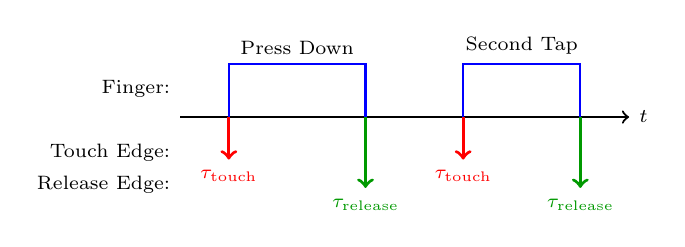
\begin{tikzpicture}[x=0.62cm, y=0.45cm]
    % Time axis
    \draw[->, thick] (0,0) -- (9.2,0) node[right] {\scriptsize $t$};
    
    % Finger Contact
    \draw[thick, blue] (1,0) -- (1,1.5) -- (3.8,1.5) -- (3.8,0);
    \node[above] at (2.4,1.5) {\scriptsize Press Down};
    
    \draw[thick, blue] (5.8,0) -- (5.8,1.5) -- (8.2,1.5) -- (8.2,0);
    \node[above] at (7.0,1.5) {\scriptsize Second Tap};
    
    % Touch Edge Pulse
    \draw[->, red, very thick] (1,0) -- (1,-1.2) node[below] {\scriptsize $\tau_{\text{touch}}$};
    \draw[->, red, very thick] (5.8,0) -- (5.8,-1.2) node[below] {\scriptsize $\tau_{\text{touch}}$};
    
    % Release Edge Pulse
    \draw[->, green!60!black, very thick] (3.8,0) -- (3.8,-2.0) node[below] {\scriptsize $\tau_{\text{release}}$};
    \draw[->, green!60!black, very thick] (8.2,0) -- (8.2,-2.0) node[below] {\scriptsize $\tau_{\text{release}}$};
    
    \node[left] at (0,0.8) {\scriptsize Finger:};
    \node[left] at (0,-1.0) {\scriptsize Touch Edge:};
    \node[left] at (0,-1.9) {\scriptsize Release Edge:};
\end{tikzpicture}
\caption{Temporal timing diagram: Touch Edge vs. Release Edge triggering.}
\label{fig:edges}
\end{figure}

\begin{definition}[Trigger Invariant]
Let $e(t) \in \{0, 1\}$ represent the physical or optical contact state.
\begin{align}
\tau_{\text{touch}}   &= \{ t \mid e(t^-) = 0 \land e(t^+) = 1 \} \\
\tau_{\text{release}} &= \{ t \mid e(t^-) = 1 \land e(t^+) = 0 \land p(t) \in \Omega_{\text{bounds}} \}
\end{align}
where $p(t)$ is the pointer or contact coordinate and $\Omega_{\text{bounds}}$ is the bounding rectangle of the control.
\end{definition}

\textbf{Rule 9-1 (Confirmation Safety):} All irreversible, committing, or hazardous operations (e.g., \emph{Execute}, \emph{Format}, \emph{Delete}) must strictly bind to $\tau_{\text{release}}$. If the user presses the button, realizes an error, and drags the cursor outside $\Omega_{\text{bounds}}$ prior to release, the action is aborted without state mutation.

%-------------------------------------------------------------------------
\section{Spatial Layout and the Standard Action Triad}
\label{sec:layout}

TRON HMI mandates deterministic spatial relationships based on human ergonomic motor polarity (Chapter 11).

\subsection{Standard Switch Layout Order}
For any dialog, panel, or appliance execution block, interactive switches must be positioned in strict order along the horizontal reading axis:
\begin{equation}
\text{[Cancel]} \;\longrightarrow\; \text{[Default]} \;\longrightarrow\; \text{[Start/Exec]}
\end{equation}
\begin{itemize}[leftmargin=*]
    \item \textbf{Cancel (\ja{取り消し}):} Positioned at the leftmost position (or top in vertical stacks), allowing immediate escape.
    \item \textbf{Default (\ja{標準設定}):} Centered, restoring calibrated factory parameters.
    \item \textbf{Start / Execute (\ja{実行}):} Positioned at the rightmost position (or bottom), preventing accidental launch.
\end{itemize}

\subsection{Label Placement and Hand Non-Occlusion}
\textbf{Guideline 11-17 (Occlusion Prevention):} To prevent the operator's hand from obstructing numeric scales during adjustment:
\begin{itemize}[leftmargin=*]
    \item For horizontal slide controls ($\leftrightarrow$), labels and graduation marks must reside \textbf{above} the track.
    \item For vertical slide controls ($\updownarrow$), labels must reside on the \textbf{left} side for right-handed ergonomic clearance.
\end{itemize}

\subsection{Enableware and Three-Color Status Indication}
Accessibility (\emph{Enableware -- \ja{イネーブルウェア}}) is embedded directly into the structural specification:
\begin{itemize}[leftmargin=*]
    \item \textbf{Tactile Homemark (\ja{ボッチ}):} Raised tactile homemark dots on center keys (key `5' on 10-key pads and primary power switches).
    \item \textbf{Three-Color Chromatic Protocol (Chapter 9):} Green (Normal/Active), Amber (Standby/Transit), and Red (Stop/Error).
    \item \textbf{Acoustic Redundancy (\ja{音による確認}):} Standardized audio earcons: confirmation chimes ($880\,\text{Hz}$), parameter clicks ($440\,\text{Hz}$), and error alerts ($220\,\text{Hz}$).
\end{itemize}

%-------------------------------------------------------------------------
\section{The Universal Controller (\texorpdfstring{\ja{万能コントローラ}}{Universal Controller})}
\label{sec:universal}

To unify appliance control without requiring pointing devices, TRON HMI specifies the \textbf{Universal Controller} (Chapter 7)---a canonical 7-key remote navigation model. It establishes an invariant directional d-pad coupled with distinct confirmation (\texttt{Execute}) and escape (\texttt{Cancel}) switches, avoiding nested modal submenus.

\begin{figure}[htbp]
\centering
\begin{tikzpicture}[scale=0.58]
    % Remote Body
    \draw[fill=gray!20, rounded corners=4pt, line width=0.8pt] (0,0) rectangle (3.2,4.4);
    \node at (1.6,4.05) {\textbf{\scriptsize \ja{万能コントローラ}}};

    % D-Pad Up
    \draw[fill=gray!40, rounded corners=2pt] (1.1,3.0) rectangle (2.1,3.6);
    \node at (1.6,3.3) {\footnotesize $\blacktriangle$};
    \node[right] at (2.2,3.3) {\tiny Prev Item (\ja{前})};

    % D-Pad Down
    \draw[fill=gray!40, rounded corners=2pt] (1.1,1.7) rectangle (2.1,2.3);
    \node at (1.6,2.0) {\footnotesize $\blacktriangledown$};
    \node[right] at (2.2,2.0) {\tiny Next Item (\ja{次})};

    % D-Pad Left
    \draw[fill=gray!40, rounded corners=2pt] (0.35,2.35) rectangle (1.35,2.95);
    \node at (0.85,2.65) {\footnotesize $\blacktriangleleft$};

    % D-Pad Right
    \draw[fill=gray!40, rounded corners=2pt] (1.85,2.35) rectangle (2.85,2.95);
    \node at (2.35,2.65) {\footnotesize $\blacktriangleright$};

    % Cancel [X]
    \draw[fill=red!70, rounded corners=2pt] (0.35,0.9) rectangle (1.35,1.45);
    \node[white] at (0.85,1.17) {\textbf{\footnotesize X}};
    \node[below] at (0.85,0.9) {\tiny Cancel (\ja{取})};

    % Execute [O]
    \draw[fill=green!60!black, rounded corners=2pt] (1.85,0.9) rectangle (2.85,1.45);
    \node[white] at (2.35,1.17) {\textbf{\footnotesize O}};
    \node[below] at (2.35,0.9) {\tiny Exec (\ja{実})};

    % Command [Naming]
    \draw[fill=gray!30, rounded corners=2pt] (0.9,0.25) rectangle (2.3,0.65);
    \node at (1.6,0.45) {\tiny \ja{命名} (Menu)};
\end{tikzpicture}
\caption{TRON 7-Key Universal Controller Remote Model (Chapter 7).}
\label{fig:remote}
\end{figure}

\subsection{Current Item Traversal Algebra}
The Universal Controller navigates a discrete set of panel controls $\mathcal{P} = \{c_0, c_1, \dots, c_{n-1}\}$ through an active focus pointer index $\kappa \in [0, n-1]$ known as the \textbf{Current Item} (\ja{カレント項目}):
\begin{align}
\kappa_{t+1} &= (\kappa_t \pm 1) \bmod n \\
v(\kappa)_{t+1} &= \operatorname{clamp}(v(\kappa)_t \pm \delta, v_{\min}, v_{\max})
\end{align}

This guarantees complete operational capability for any multi-item panel over simple 4-way infrared remotes, rotary encoder pulses, or single-switch accessibility scanning.

%-------------------------------------------------------------------------
\section{State Machine Transitions and Modelessness}
\label{sec:fsm}

TRON HMI formalizes four fundamental transition models between interface states (Chapter 12):

\begin{figure}[htbp]
\centering
\begin{tikzpicture}[->, >=stealth, auto, every node/.style={font=\scriptsize}]
    \node[draw, rounded corners, fill=blue!10, text width=1.6cm, align=center] (play) {\textbf{Playback}\\\ja{再生状態}};
    \path (play) edge[loop right] node[text width=2.4cm, align=left] {\textbf{Modeless Adjustments:}\\\tiny $\bullet$ Volume (\ja{音量})\\\tiny $\bullet$ Tone (\ja{音質})\\\tiny $\bullet$ Balance (\ja{バランス})} (play);
\end{tikzpicture}
\caption{Modeless parallel state transition model (Figure 12-3).}
\label{fig:modeless}
\end{figure}

\begin{enumerate}[leftmargin=*]
    \item \textbf{Sequential Transitions (\ja{逐次型遷移}):} Linear stage progression ($S_0 \to S_1 \to S_2$) with mandatory step-back capability (\emph{Guideline 12-2}).
    \item \textbf{Selective Transitions (\ja{選択型遷移}):} Branching choice dispatching to mutually exclusive operational modes.
    \item \textbf{Parallel / Modeless Transitions (\ja{並列型遷移}):} Independent parameter adjustment without mode shifts (\emph{Guideline 12-1}).
    \item \textbf{Interrupt Transitions (\ja{割込型遷移}):} Asynchronous emergency abort or reset transition from any state directly into the safe quiescent state: $\forall s \in \mathcal{S}, \;\delta(s, \text{EVENT\_CANCEL}) = S_{\text{idle}}$.
\end{enumerate}

%-------------------------------------------------------------------------
\section{Cleanroom Implementation and Verification}
\label{sec:impl}

To satisfy rigorous aerospace and embedded systems standards (specifically MISRA-C:2012 guidelines and NASA JPL Safety-Critical Software Rules~\cite{holzmann2006jpl}), our cleanroom implementation (\texttt{libhmi}) is engineered under strict determinism and reliability principles:

\begin{enumerate}[leftmargin=*]
    \item \textbf{Zero Dynamic Memory Allocation (JPL Rule 3):} Dynamic heap allocations (\texttt{malloc}, \texttt{calloc}, \texttt{free}) are strictly forbidden during runtime operation after initial boot. All data structures (\texttt{HMI\_PANEL}, \texttt{HMI\_CTRL}) allocate flat, statically bounded arrays (\texttt{HMI\_PANEL\_MAX\_CTRLS = 32}, fixed 64-byte title strings). This completely eliminates heap fragmentation, memory exhaustion faults, and non-deterministic garbage collection or allocation latency in critical control loops.
    \item \textbf{Bounded Deterministic Event Dispatch (MISRA Dir 4.1):} Pointer coordinates and remote keypad events are evaluated via pure integer bounding-box intersections with a strict upper bound $O(N)$ where $N \le 32$. This guarantees bounded worst-case execution time (WCET) and zero dispatch jitter during high-frequency hardware interrupt servicing.
    \item \textbf{Reentrant and Isolated State Model:} Control state mutations occur exclusively via designated event-handler callbacks. Pointer capture and focus indices are managed within local panel state, isolating interactive components from global workstation state.
    \item \textbf{Decoupled Composite Rendering Pipeline:} Control logic executes synchronously on input events, marking invalidated bounding regions. The presentation layer performs dirty-rectangle composite blitting onto the display context (\texttt{GDEV}), strictly preserving model-view separation and avoiding redundant graphical re-draws.
\end{enumerate}

The core C99 container definition establishing these deterministic memory invariants and control slots is formally defined in Listing~\ref{lst:panel}:

\begin{lstlisting}[language=C, caption={Deterministic Panel Container in include/btron/hmi.h}, label={lst:panel}]
#define HMI_PANEL_MAX_CTRLS 32

typedef struct HMI_PANEL {
    ID          id;
    char        title[64];
    RECT        bounds;
    COLOR       bg_color;
    HMI_CTRL    controls[HMI_PANEL_MAX_CTRLS];
    int         num_controls;
    int         focused_index;  /* Current Item */
    BOOL        show_remote;
    void        (*on_paint_custom)(struct HMI_PANEL *panel, GDEV *dev);
} HMI_PANEL;
\end{lstlisting}

\subsection{Canonical Showcase: SONY TC-K777ES Audio Deck}
We realized a canonical workstation application (\texttt{src/apps/audio\_player.c}) modeling the classic 3-Head SONY TC-K777ES stereo cassette deck. The application integrates:
\begin{itemize}[leftmargin=*]
    \item Dual spinning tape spools with dynamic tape thickness transfer.
    \item 12-segment fluorescent VU bar meters with falling peak indicators (decay rate $\Delta v_{\text{peak}} = -2\,\text{dB}/\text{frame}$).
    \item Rotary Master Volume, Bass, Treble, and Balance potentiometers ($270^\circ$ angular sweep).
    \item Pop-up Universal Controller remote navigation overlay.
\end{itemize}

\begin{table}[htbp]
\centering
\caption{TRON HMI Automated Unit Test Results}
\label{tab:tests}
\resizebox{\columnwidth}{!}{
\begin{tabular}{@{}lcc@{}}
\toprule
\textbf{Test Module / Component} & \textbf{Assertions} & \textbf{Pass Rate} \\ \midrule
Panel Lifecycle \& Memory Layout & 5 & 100.0\% \\
Switches \& Touch/Release Triggers & 10 & 100.0\% \\
Up/Down Steppers \& Radio Matrices & 7 & 100.0\% \\
Continuous Volumes \& Rotary Dials & 5 & 100.0\% \\
Universal Controller \& Focus Algebra & 6 & 100.0\% \\ \midrule
\textbf{Total Test Suite Coverage} & \textbf{33 / 33} & \textbf{100.0\%} \\ \bottomrule
\end{tabular}
}
\end{table}

%-------------------------------------------------------------------------
\section{Conclusion}
\label{sec:conclusion}

The TRON Human-Machine Interface specification establishes a mathematically rigorous, culturally neutral, and ergonomically sound foundation for human-machine collaboration across embedded appliances and workstation environments. By formalizing Touch/Release edge mechanics, the Standard Action Triad, modeless parallel state machines, and the 7-key Universal Controller, our cleanroom implementation demonstrates that operational uniformity can be achieved without compromising industrial aesthetic freedom.

%-------------------------------------------------------------------------
\begin{thebibliography}{99}

\bibitem{sakamura1987tron}
K.~Sakamura, ``The TRON Project,'' \emph{IEEE Micro}, vol.~7, no.~2, pp.~8--14, Apr. 1987.

\bibitem{sakamura1993hmi}
K.~Sakamura, \emph{TRON Human-Machine Interface Specifications}, Personal Media Corporation, Tokyo, Japan, 1993.

\bibitem{sakamura1997btron}
K.~Sakamura, \emph{BTRON3 SPEC 3.20: Business TRON Workstation Specification}, TRON Association, Tokyo, Japan, 1997.

\bibitem{holzmann2006jpl}
G.~J.~Holzmann, ``The Power of 10: Rules for Developing Safety-Critical Code,'' \emph{IEEE Computer}, vol.~39, no.~6, pp.~95--97, Jun. 2006.

\bibitem{norman2013design}
D.~A.~Norman, \emph{The Design of Everyday Things: Revised and Expanded Edition}, Basic Books, New York, 2013.

\end{thebibliography}

\end{document}
